\section{Questions à choix multiples (3 points)}\label{qcm}
Pour chaque question, choisir la (ou les) bonne(s) réponse(s).

\begin{questions}
	\question[1] Dans la situation ci-dessous, l'action qui déforme le trampoline est :
	
	\begin{multicols}{2}
	
		\begin{center}
			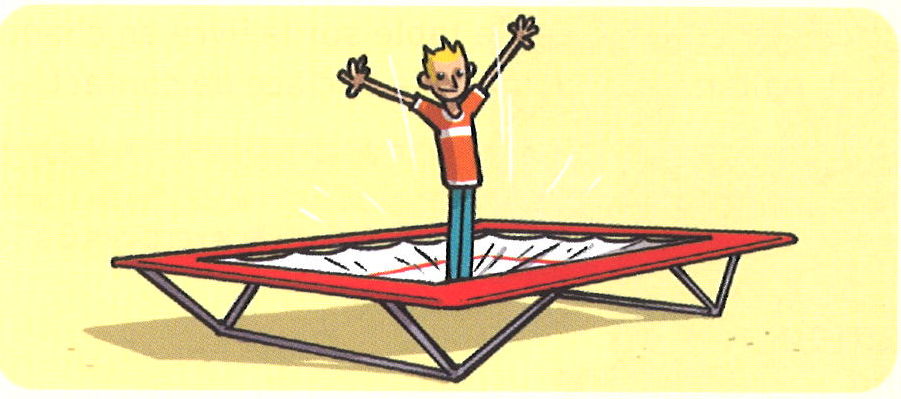
\includegraphics[scale=0.3]{trampo}	
		\end{center}
	
	
		\begin{checkboxes}
			\correctchoice celle exercée par l'enfant sur le trampoline.
			\choice celle exercée par le trampoline sur l'enfant.
			\choice le poids du trampoline.
		\end{checkboxes}
	\end{multicols}

	\question[1] Dans la situation ci-dessous, la force modélisée par la flèche est celle exercée :
	
	\begin{multicols}{2}
		
			
		\begin{center}
			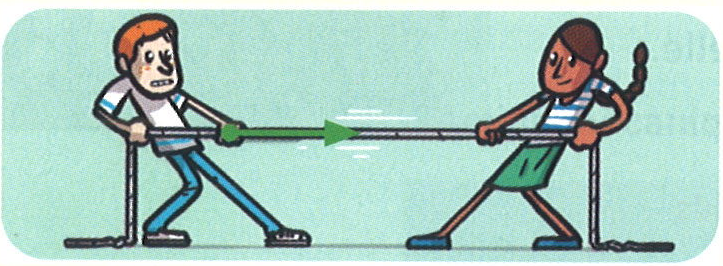
\includegraphics[scale=0.3]{corde}
		\end{center}
		\begin{checkboxes}
			\choice par la fille sur le garçon.
			\correctchoice par la corde sur le garçon.
			\choice par la fille sur la corde.
		\end{checkboxes}
		
	\end{multicols}

	\question[1] Dans la situation ci-dessous, le plongeur est soumis :
	
	\begin{multicols}{2}
		
		
		\begin{center}
			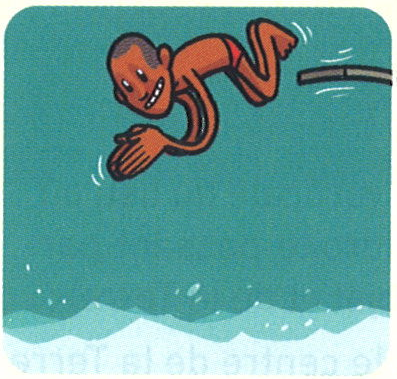
\includegraphics[scale=0.3]{plong}
		\end{center}
		\begin{checkboxes}
			\choice à l'action exercée par le plongeoir.
			\correctchoice à l'action exercée par la Terre.
			\correctchoice à l'action exercée par l'air.
		\end{checkboxes}
	\end{multicols}

\end{questions}